% ============================================================
% DMGR — Memory Efficiency Section  (concise, IEEE conference)
% Usage: % ============================================================
% DMGR — Memory Efficiency Section  (concise, IEEE conference)
% Usage: % ============================================================
% DMGR — Memory Efficiency Section  (concise, IEEE conference)
% Usage: % ============================================================
% DMGR — Memory Efficiency Section  (concise, IEEE conference)
% Usage: \input{dmgr}
% Requires: booktabs, graphicx (already in main.tex)
% Figure: figures/vram_memory_scaling.pdf
% ============================================================

\subsection{Memory Efficiency During Generation}

While inference memory scaling is widely discussed in the context of KV-cache
optimisation~\cite{Luohe2024Keep, Nawrot2024Dynamic, Li2024SnapKV}, existing
work typically reports raw measurements at fixed lengths or qualitative
O($L$) complexity arguments rather than a formalised empirical rate.
Following this practice, we define \textit{Decode Memory Growth Rate} (DMGR)
as a concrete scalar metric suitable for cross-architecture comparison:

\begin{equation}
  \mathrm{DMGR} = \frac{M(L_2) - M(L_1)}{L_2 - L_1}, \quad
  M(L) = \text{Peak VRAM}(L) - \text{Idle VRAM}
  \label{eq:dmgr}
\end{equation}

\noindent where $M(L)$ is peak incremental VRAM at generation length $L$,
isolating runtime overhead from the static model footprint.
A DMGR of zero indicates constant memory; a positive value indicates
length-dependent growth, reported in MB per 1k generated tokens (or steps).
We measure $\mathrm{DMGR}_{1\mathrm{k}\to12\mathrm{k}}$ at lengths
$\{1\mathrm{k}, 2\mathrm{k}, 4\mathrm{k}, 8\mathrm{k}, 12\mathrm{k}\}$
on an NVIDIA RTX 6000 Ada (49\,GB), monitoring VRAM via NVML at 50\,ms
intervals with a fresh process per measurement to avoid cross-contamination.

Table~\ref{tab:dmgr} and Fig.~\ref{fig:vram_scaling} summarise the results.

\begin{table}[h]
  \centering
  \caption{Peak Incremental VRAM (MB) and DMGR.
           xLSTM values use the PyTorch allocator.
           \textsuperscript{\dag}Lookback RNN values reflect TensorFlow's
           fixed pre-allocated memory pool (sequence-length independent).}
  \label{tab:dmgr}
  \setlength{\tabcolsep}{3.5pt}
  \begin{tabular}{lrrrrrr}
    \toprule
    \textbf{Model} &
    \textbf{1k} & \textbf{2k} & \textbf{4k} & \textbf{8k} & \textbf{12k} &
    \textbf{DMGR} \\
    & \multicolumn{5}{c}{\footnotesize(MB)} & \footnotesize(MB/1k) \\
    \midrule
    Lookback RNN  & \multicolumn{5}{c}{47,171\textsuperscript{\dag} (flat)} & 0.00 \\
    xLSTM (ours)  & 20.9 & 21.4 & 22.4 & 24.3 & 26.3 & 0.49 \\
    Museformer    & 190  & 956  & 6,250 & 31,874 & 47,986 & 4,345 \\
    \bottomrule
  \end{tabular}
\end{table}

\begin{figure}[h]
  \centering
  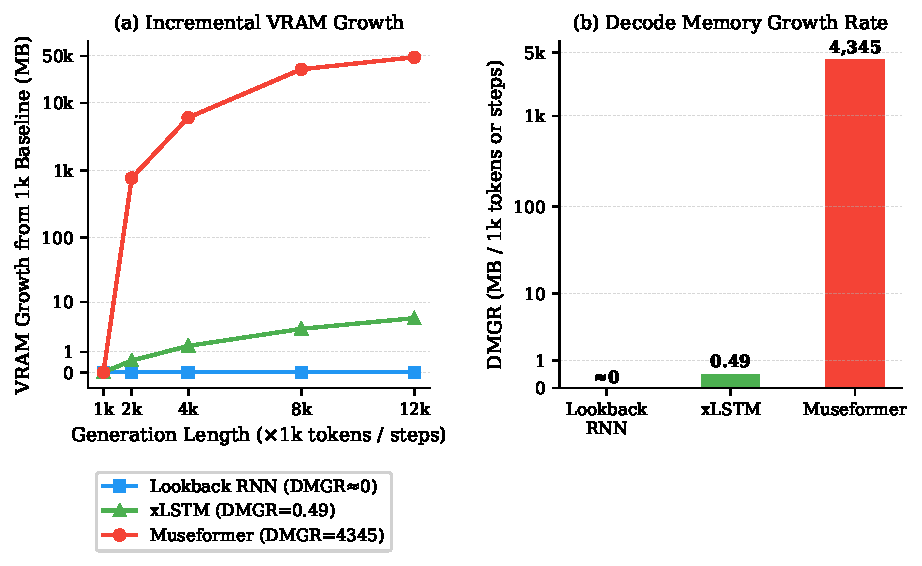
\includegraphics[width=\columnwidth]{figures/vram_memory_scaling.pdf}
  \caption{Memory scaling across three models.
           \textbf{(a)}~VRAM growth above the 1k baseline
           ($\ln(1{+}x)$ scale; flat line = constant memory).
           \textbf{(b)}~DMGR comparison ($\ln(1{+}x)$ scale; lower is better).}
  \label{fig:vram_scaling}
\end{figure}

The results reveal three distinct regimes.
Lookback RNN achieves DMGR\,=\,0, consistent with its fixed recurrent hidden
state; the large absolute value in Table~\ref{tab:dmgr} is TensorFlow's
pre-allocated pool, not sequence-dependent overhead.
xLSTM achieves a near-constant profile (DMGR\,=\,0.49\,MB/1k tokens),
growing only 5.4\,MB across the full 1k--12k span, consistent with
recurrent-state inference where the mLSTM state is updated in place rather
than accumulated over the full context.
Museformer, by contrast, exhibits super-linear growth
(DMGR\,=\,4{,}345\,MB/1k tokens), exhausting nearly all 49\,GB of VRAM at
12k tokens due to its block-sparse attention over an expanding token history.
xLSTM's DMGR is approximately $\mathbf{8{,}877{\times}}$ lower than Museformer's,
demonstrating that recurrent-state inference provides a decisive memory
advantage for long-form generation without sacrificing the richer
multi-track representations that Lookback RNN cannot produce.

% Requires: booktabs, graphicx (already in main.tex)
% Figure: figures/vram_memory_scaling.pdf
% ============================================================

\subsection{Memory Efficiency During Generation}

While inference memory scaling is widely discussed in the context of KV-cache
optimisation~\cite{Luohe2024Keep, Nawrot2024Dynamic, Li2024SnapKV}, existing
work typically reports raw measurements at fixed lengths or qualitative
O($L$) complexity arguments rather than a formalised empirical rate.
Following this practice, we define \textit{Decode Memory Growth Rate} (DMGR)
as a concrete scalar metric suitable for cross-architecture comparison:

\begin{equation}
  \mathrm{DMGR} = \frac{M(L_2) - M(L_1)}{L_2 - L_1}, \quad
  M(L) = \text{Peak VRAM}(L) - \text{Idle VRAM}
  \label{eq:dmgr}
\end{equation}

\noindent where $M(L)$ is peak incremental VRAM at generation length $L$,
isolating runtime overhead from the static model footprint.
A DMGR of zero indicates constant memory; a positive value indicates
length-dependent growth, reported in MB per 1k generated tokens (or steps).
We measure $\mathrm{DMGR}_{1\mathrm{k}\to12\mathrm{k}}$ at lengths
$\{1\mathrm{k}, 2\mathrm{k}, 4\mathrm{k}, 8\mathrm{k}, 12\mathrm{k}\}$
on an NVIDIA RTX 6000 Ada (49\,GB), monitoring VRAM via NVML at 50\,ms
intervals with a fresh process per measurement to avoid cross-contamination.

Table~\ref{tab:dmgr} and Fig.~\ref{fig:vram_scaling} summarise the results.

\begin{table}[h]
  \centering
  \caption{Peak Incremental VRAM (MB) and DMGR.
           xLSTM values use the PyTorch allocator.
           \textsuperscript{\dag}Lookback RNN values reflect TensorFlow's
           fixed pre-allocated memory pool (sequence-length independent).}
  \label{tab:dmgr}
  \setlength{\tabcolsep}{3.5pt}
  \begin{tabular}{lrrrrrr}
    \toprule
    \textbf{Model} &
    \textbf{1k} & \textbf{2k} & \textbf{4k} & \textbf{8k} & \textbf{12k} &
    \textbf{DMGR} \\
    & \multicolumn{5}{c}{\footnotesize(MB)} & \footnotesize(MB/1k) \\
    \midrule
    Lookback RNN  & \multicolumn{5}{c}{47,171\textsuperscript{\dag} (flat)} & 0.00 \\
    xLSTM (ours)  & 20.9 & 21.4 & 22.4 & 24.3 & 26.3 & 0.49 \\
    Museformer    & 190  & 956  & 6,250 & 31,874 & 47,986 & 4,345 \\
    \bottomrule
  \end{tabular}
\end{table}

\begin{figure}[h]
  \centering
  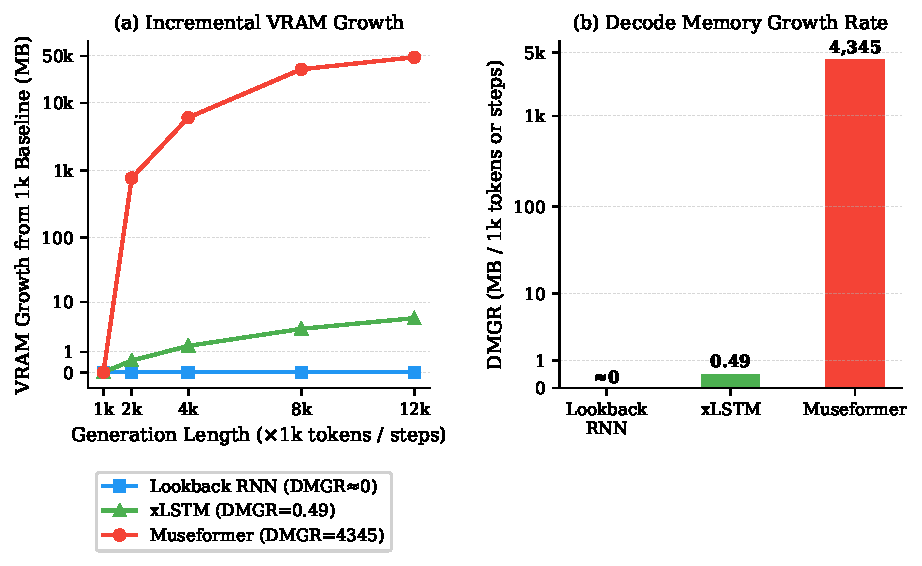
\includegraphics[width=\columnwidth]{figures/vram_memory_scaling.pdf}
  \caption{Memory scaling across three models.
           \textbf{(a)}~VRAM growth above the 1k baseline
           ($\ln(1{+}x)$ scale; flat line = constant memory).
           \textbf{(b)}~DMGR comparison ($\ln(1{+}x)$ scale; lower is better).}
  \label{fig:vram_scaling}
\end{figure}

The results reveal three distinct regimes.
Lookback RNN achieves DMGR\,=\,0, consistent with its fixed recurrent hidden
state; the large absolute value in Table~\ref{tab:dmgr} is TensorFlow's
pre-allocated pool, not sequence-dependent overhead.
xLSTM achieves a near-constant profile (DMGR\,=\,0.49\,MB/1k tokens),
growing only 5.4\,MB across the full 1k--12k span, consistent with
recurrent-state inference where the mLSTM state is updated in place rather
than accumulated over the full context.
Museformer, by contrast, exhibits super-linear growth
(DMGR\,=\,4{,}345\,MB/1k tokens), exhausting nearly all 49\,GB of VRAM at
12k tokens due to its block-sparse attention over an expanding token history.
xLSTM's DMGR is approximately $\mathbf{8{,}877{\times}}$ lower than Museformer's,
demonstrating that recurrent-state inference provides a decisive memory
advantage for long-form generation without sacrificing the richer
multi-track representations that Lookback RNN cannot produce.

% Requires: booktabs, graphicx (already in main.tex)
% Figure: figures/vram_memory_scaling.pdf
% ============================================================

\subsection{Memory Efficiency During Generation}

While inference memory scaling is widely discussed in the context of KV-cache
optimisation~\cite{Luohe2024Keep, Nawrot2024Dynamic, Li2024SnapKV}, existing
work typically reports raw measurements at fixed lengths or qualitative
O($L$) complexity arguments rather than a formalised empirical rate.
Following this practice, we define \textit{Decode Memory Growth Rate} (DMGR)
as a concrete scalar metric suitable for cross-architecture comparison:

\begin{equation}
  \mathrm{DMGR} = \frac{M(L_2) - M(L_1)}{L_2 - L_1}, \quad
  M(L) = \text{Peak VRAM}(L) - \text{Idle VRAM}
  \label{eq:dmgr}
\end{equation}

\noindent where $M(L)$ is peak incremental VRAM at generation length $L$,
isolating runtime overhead from the static model footprint.
A DMGR of zero indicates constant memory; a positive value indicates
length-dependent growth, reported in MB per 1k generated tokens (or steps).
We measure $\mathrm{DMGR}_{1\mathrm{k}\to12\mathrm{k}}$ at lengths
$\{1\mathrm{k}, 2\mathrm{k}, 4\mathrm{k}, 8\mathrm{k}, 12\mathrm{k}\}$
on an NVIDIA RTX 6000 Ada (49\,GB), monitoring VRAM via NVML at 50\,ms
intervals with a fresh process per measurement to avoid cross-contamination.

Table~\ref{tab:dmgr} and Fig.~\ref{fig:vram_scaling} summarise the results.

\begin{table}[h]
  \centering
  \caption{Peak Incremental VRAM (MB) and DMGR.
           xLSTM values use the PyTorch allocator.
           \textsuperscript{\dag}Lookback RNN values reflect TensorFlow's
           fixed pre-allocated memory pool (sequence-length independent).}
  \label{tab:dmgr}
  \setlength{\tabcolsep}{3.5pt}
  \begin{tabular}{lrrrrrr}
    \toprule
    \textbf{Model} &
    \textbf{1k} & \textbf{2k} & \textbf{4k} & \textbf{8k} & \textbf{12k} &
    \textbf{DMGR} \\
    & \multicolumn{5}{c}{\footnotesize(MB)} & \footnotesize(MB/1k) \\
    \midrule
    Lookback RNN  & \multicolumn{5}{c}{47,171\textsuperscript{\dag} (flat)} & 0.00 \\
    xLSTM (ours)  & 20.9 & 21.4 & 22.4 & 24.3 & 26.3 & 0.49 \\
    Museformer    & 190  & 956  & 6,250 & 31,874 & 47,986 & 4,345 \\
    \bottomrule
  \end{tabular}
\end{table}

\begin{figure}[h]
  \centering
  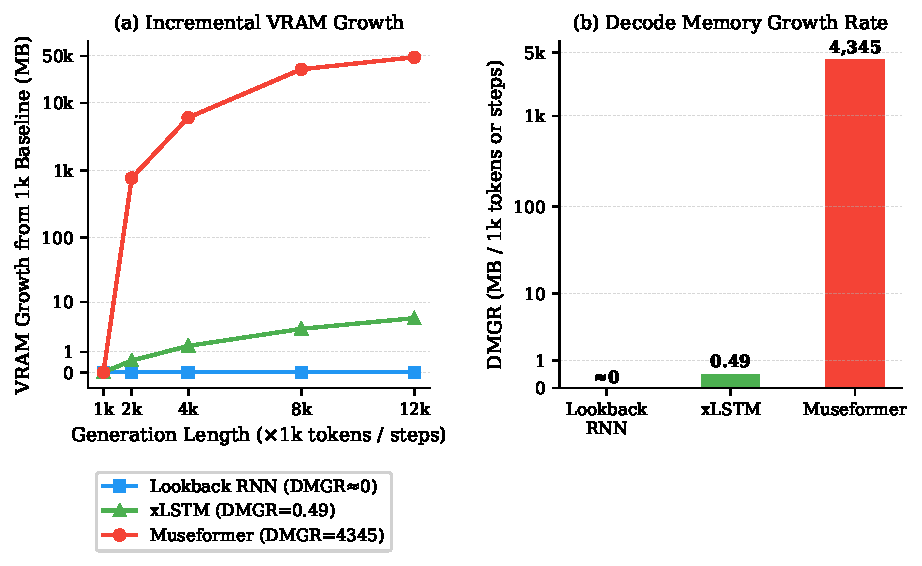
\includegraphics[width=\columnwidth]{figures/vram_memory_scaling.pdf}
  \caption{Memory scaling across three models.
           \textbf{(a)}~VRAM growth above the 1k baseline
           ($\ln(1{+}x)$ scale; flat line = constant memory).
           \textbf{(b)}~DMGR comparison ($\ln(1{+}x)$ scale; lower is better).}
  \label{fig:vram_scaling}
\end{figure}

The results reveal three distinct regimes.
Lookback RNN achieves DMGR\,=\,0, consistent with its fixed recurrent hidden
state; the large absolute value in Table~\ref{tab:dmgr} is TensorFlow's
pre-allocated pool, not sequence-dependent overhead.
xLSTM achieves a near-constant profile (DMGR\,=\,0.49\,MB/1k tokens),
growing only 5.4\,MB across the full 1k--12k span, consistent with
recurrent-state inference where the mLSTM state is updated in place rather
than accumulated over the full context.
Museformer, by contrast, exhibits super-linear growth
(DMGR\,=\,4{,}345\,MB/1k tokens), exhausting nearly all 49\,GB of VRAM at
12k tokens due to its block-sparse attention over an expanding token history.
xLSTM's DMGR is approximately $\mathbf{8{,}877{\times}}$ lower than Museformer's,
demonstrating that recurrent-state inference provides a decisive memory
advantage for long-form generation without sacrificing the richer
multi-track representations that Lookback RNN cannot produce.

% Requires: booktabs, graphicx (already in main.tex)
% Figure: figures/vram_memory_scaling.pdf
% ============================================================

\subsection{Memory Efficiency During Generation}

While inference memory scaling is widely discussed in the context of KV-cache
optimisation~\cite{Luohe2024Keep, Nawrot2024Dynamic, Li2024SnapKV}, existing
work typically reports raw measurements at fixed lengths or qualitative
O($L$) complexity arguments rather than a formalised empirical rate.
Following this practice, we define \textit{Decode Memory Growth Rate} (DMGR)
as a concrete scalar metric suitable for cross-architecture comparison:

\begin{equation}
  \mathrm{DMGR} = \frac{M(L_2) - M(L_1)}{L_2 - L_1}, \quad
  M(L) = \text{Peak VRAM}(L) - \text{Idle VRAM}
  \label{eq:dmgr}
\end{equation}

\noindent where $M(L)$ is peak incremental VRAM at generation length $L$,
isolating runtime overhead from the static model footprint.
A DMGR of zero indicates constant memory; a positive value indicates
length-dependent growth, reported in MB per 1k generated tokens (or steps).
We measure $\mathrm{DMGR}_{1\mathrm{k}\to12\mathrm{k}}$ at lengths
$\{1\mathrm{k}, 2\mathrm{k}, 4\mathrm{k}, 8\mathrm{k}, 12\mathrm{k}\}$
on an NVIDIA RTX 6000 Ada (49\,GB), monitoring VRAM via NVML at 50\,ms
intervals with a fresh process per measurement to avoid cross-contamination.

Table~\ref{tab:dmgr} and Fig.~\ref{fig:vram_scaling} summarise the results.

\begin{table}[h]
  \centering
  \caption{Peak Incremental VRAM (MB) and DMGR.
           xLSTM values use the PyTorch allocator.
           \textsuperscript{\dag}Lookback RNN values reflect TensorFlow's
           fixed pre-allocated memory pool (sequence-length independent).}
  \label{tab:dmgr}
  \setlength{\tabcolsep}{3.5pt}
  \begin{tabular}{lrrrrrr}
    \toprule
    \textbf{Model} &
    \textbf{1k} & \textbf{2k} & \textbf{4k} & \textbf{8k} & \textbf{12k} &
    \textbf{DMGR} \\
    & \multicolumn{5}{c}{\footnotesize(MB)} & \footnotesize(MB/1k) \\
    \midrule
    Lookback RNN  & \multicolumn{5}{c}{47,171\textsuperscript{\dag} (flat)} & 0.00 \\
    xLSTM (ours)  & 20.9 & 21.4 & 22.4 & 24.3 & 26.3 & 0.49 \\
    Museformer    & 190  & 956  & 6,250 & 31,874 & 47,986 & 4,345 \\
    \bottomrule
  \end{tabular}
\end{table}

\begin{figure}[h]
  \centering
  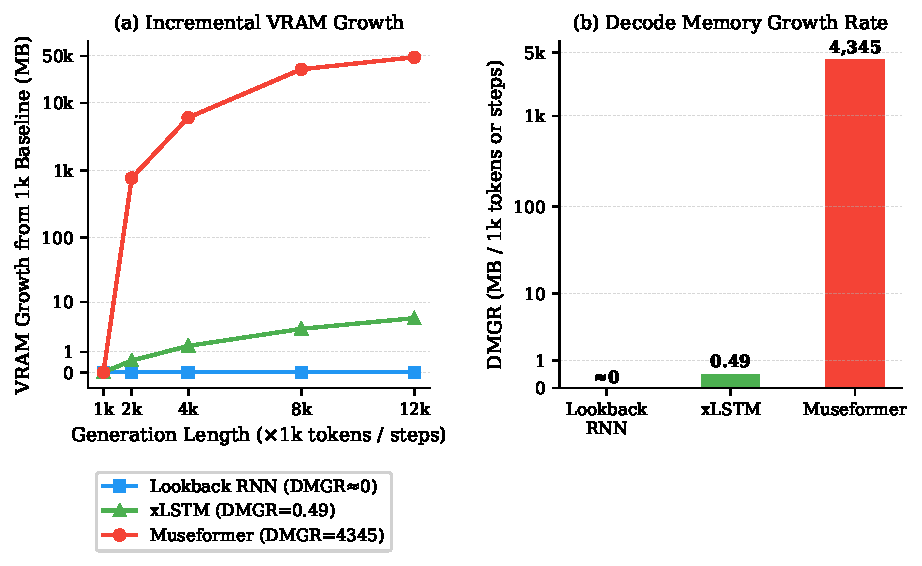
\includegraphics[width=\columnwidth]{figures/vram_memory_scaling.pdf}
  \caption{Memory scaling across three models.
           \textbf{(a)}~VRAM growth above the 1k baseline
           ($\ln(1{+}x)$ scale; flat line = constant memory).
           \textbf{(b)}~DMGR comparison ($\ln(1{+}x)$ scale; lower is better).}
  \label{fig:vram_scaling}
\end{figure}

The results reveal three distinct regimes.
Lookback RNN achieves DMGR\,=\,0, consistent with its fixed recurrent hidden
state; the large absolute value in Table~\ref{tab:dmgr} is TensorFlow's
pre-allocated pool, not sequence-dependent overhead.
xLSTM achieves a near-constant profile (DMGR\,=\,0.49\,MB/1k tokens),
growing only 5.4\,MB across the full 1k--12k span, consistent with
recurrent-state inference where the mLSTM state is updated in place rather
than accumulated over the full context.
Museformer, by contrast, exhibits super-linear growth
(DMGR\,=\,4{,}345\,MB/1k tokens), exhausting nearly all 49\,GB of VRAM at
12k tokens due to its block-sparse attention over an expanding token history.
xLSTM's DMGR is approximately $\mathbf{8{,}877{\times}}$ lower than Museformer's,
demonstrating that recurrent-state inference provides a decisive memory
advantage for long-form generation without sacrificing the richer
multi-track representations that Lookback RNN cannot produce.
